\documentclass[12pt,a4paper]{article}
\usepackage[utf8]{inputenc}
\usepackage[T1]{fontenc}
\usepackage{amsmath}
\usepackage{textcomp}

\usepackage{geometry}
\geometry{a4paper,left=25mm,right=25mm, top=2cm, bottom=2cm} 

\usepackage{graphicx} %fuer bilder

\usepackage{verbatim}


\usepackage{pgfplots}

 \usepackage{mathptmx}
 \usepackage[scaled=.90]{helvet}
 \usepackage{courier}



\usepackage{listings}
\usepackage{color}

\usepackage{float}
 
\definecolor{dkgreen}{rgb}{0,0.6,0}
\definecolor{gray}{rgb}{0.5,0.5,0.5}
\definecolor{mauve}{rgb}{0.58,0,0.82}

\pagestyle{empty}
\lstset{numbers=left,language=C++}
\lstset{showstringspaces=false,
basicstyle=\ttfamily\footnotesize,
breaklines=true,
tabsize=3,
commentstyle=\color{dkgreen},      % comment style
inputencoding={ansinew},
title=\lstname %zeigt titel der datei an
}

\usepackage{pdfpages} % fuer pdfs
\usepackage{hyperref} % fuer url

%keine einrückungen bei absatz
\parindent 0pt

\begin{document}
\title{Übung 09}
\author{Reinhard Penn, Bernhard Selymes}
\date{Mai 2015}

\normalsize

%Beginn des Dokuments

\newcommand{\Uebung}{LTLCTL}

%Angabe
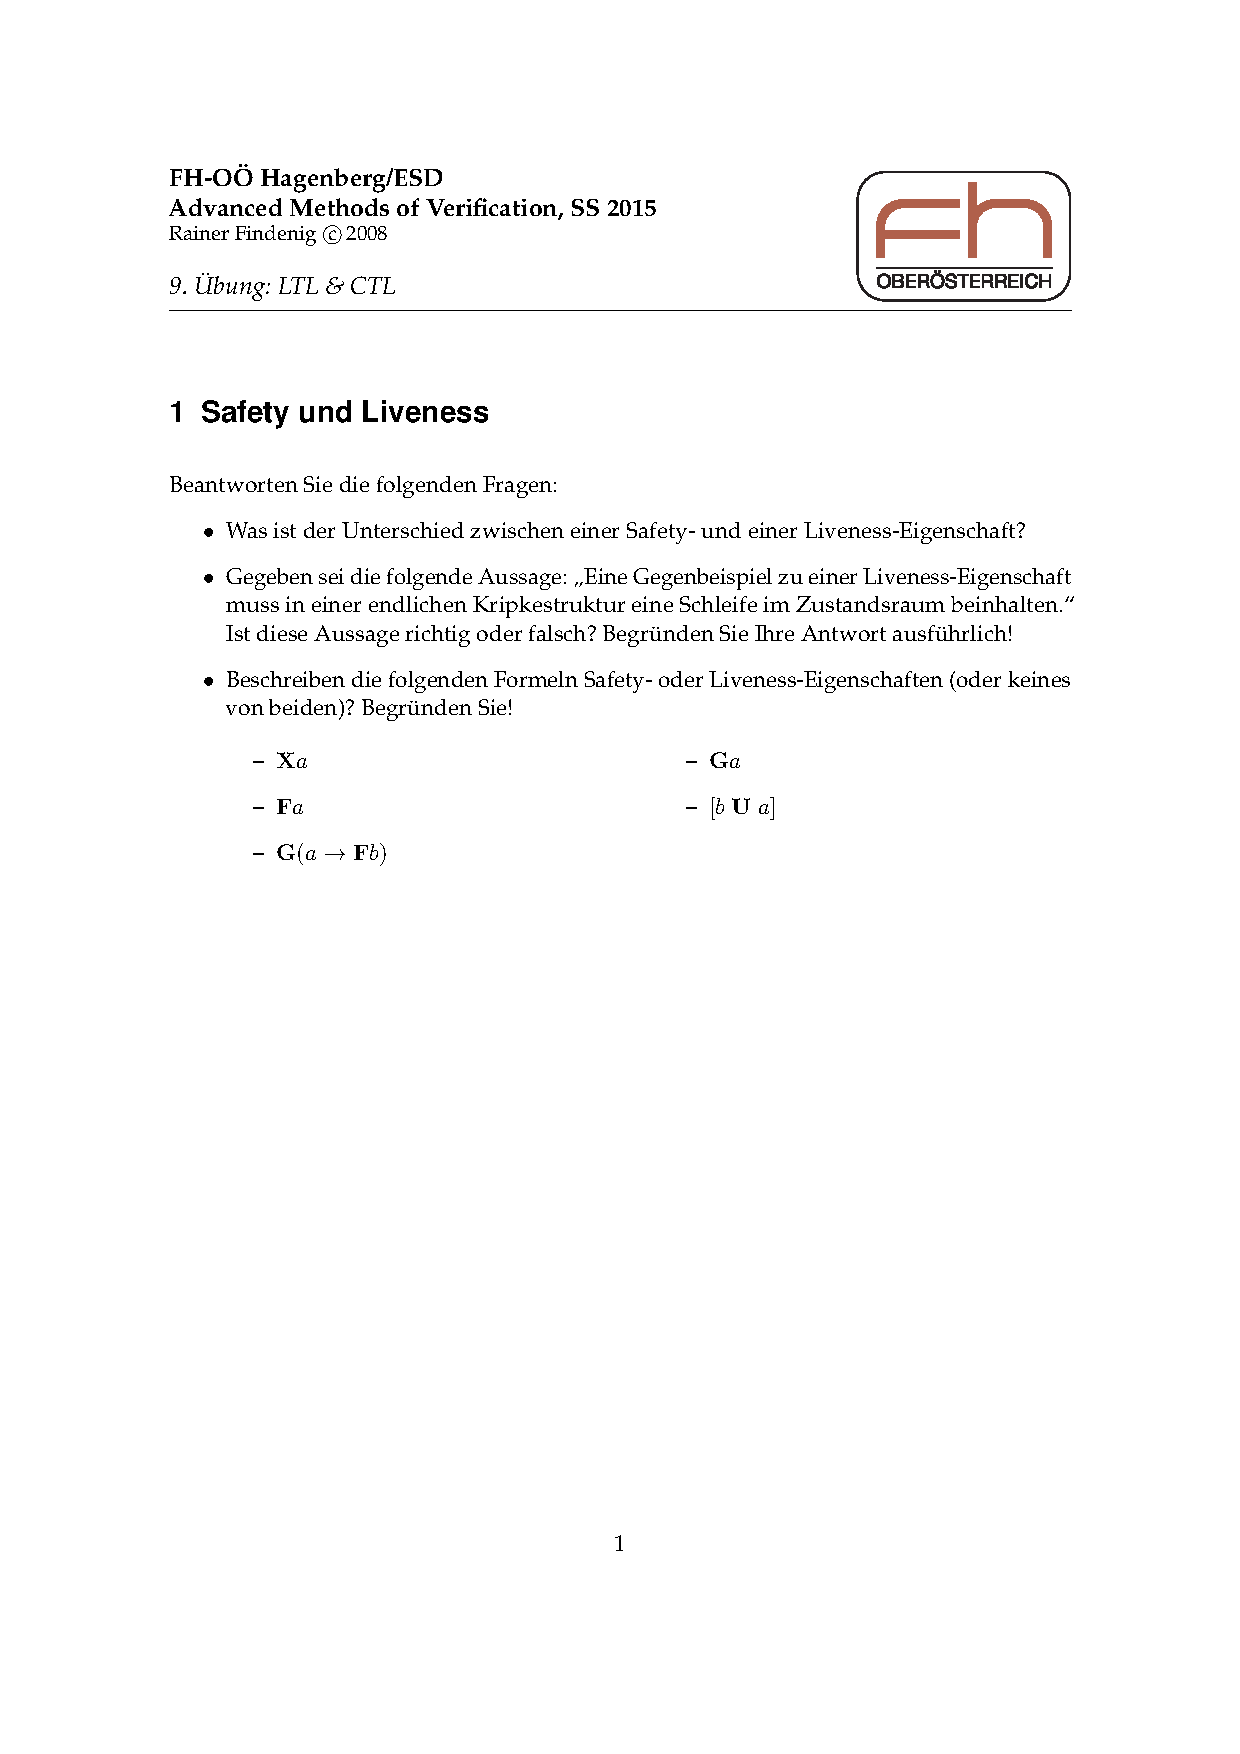
\includepdf[pages=-]{../Angabe.pdf}

\section{Beispiel 1}

\begin{itemize}
	\item Safety vs. Liveness
		\begin{itemize}
			\item Safety: Ein bestimmtes (falsches) Verhalten wird nie auftreten. Gegenbeispeispiele sind endlich.
			\item Liveness: Ein bestimmtes (richtiges) Verhalten wird schlussendlich auftreten. Gegenbeispiele sind unendlich -> kann in Simulation nicht geprüft werden.
		\end{itemize}
	\item Ja, ist richtig.\\
	Ein Gegenbeispiel zu einer Liveness-Eigenschaft ist unendlich. Die Liveness-Eigenschaft darf unendlich lang nicht erfüllt sein. Wenn man jetzt einmal davon ausgeht, dass in einem bestimmten Zustand die Liveness-Eigenschaft erfüllt ist dann muss die Kripke Struktur eine Schleife haben, die den Zustand mit der Liveness-Eigenschaft nicht beinhaltet.\\
	Beispiel:\\
	Zwei Zustände: a, b\\
	Anfangszustand: a\\
	Transitionen: a -> b, a -> a\\
	Liveness Eigenschaft: Fb\\
	In diesem Beispiel ist die Schleife von a zu a das Gegenbeispiel.
	\item Beispiele
	\begin{itemize}
		\item Safety -> Gegenbeispiel endlich
		\item Liveness -> Gegenbeispiel unendlich
		\item Liveness -> Gegenbeispiel unendlich
		\item Safety -> Gegenbeispiel endlich
		\item keines von beiden\\
		-> endliches Gegenbeispiel: $\pi = c \ldots$\\
		-> unendliches Gegenbeispiel: $\pi = b\dot{b}$
	\end{itemize}
\end{itemize}	
	
\section{Beispiel 2}

\begin{itemize}
	\item Fair
	\begin{itemize}
		\item $\pi = 01\overline{3421}$
		\item $\pi = 0342121 \ldots 342 \ldots$
	\end{itemize}
	\item Unfair
	\begin{itemize}
		\item $\pi = 03\dot{4}$
		\item $\pi = 0\overline{12}$
	\end{itemize}
\end{itemize}	
	


\end{document}
